\documentclass[a4paper]{article}
\usepackage{graphicx}
\topmargin=0.0in
\headheight=0pt
%\topmargin-0.6in
%\oddsidemargin=0.0in
%\evensidemargin=0.0in
%\marginparwidth=0.6in
%\textwidth=6.6in
%\textheight=9.8in
%NAME ADDRESS AND PHOTOGRAPH SECTION

\begin{document}
	\begin{flushleft}
		\textbf{Rohit D Khuspe} \hfill{Phone : +91 7506120970}\\
		3$^{rd}$ year BE, Electronics Engineering\hfill{Email : \underline{rohitkhuspe@gmail.com}}\\
		Fr. Conceicao Rodrigues College of Engieering\\
		Bandra West, Bandstand.\\ %\hline
		
			
	\end{flushleft}
%	\hline
		\begin{figure}[h]
			\begin{flushright}
				\vspace{-0.5in}
				%	\graphicspath{ {pictures/} }
				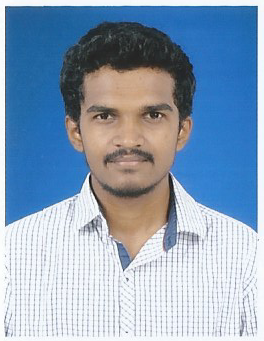
\includegraphics[width=100px]{khuspe.png}
			\end{flushright}
		\end{figure}
	
%OBJECTIVE
	\vspace{-3mm}
 \begin{flushleft}
 	\begin{Large}\textbf{Objective:}\end{Large} \hspace{0.05in} To work in a challenging environment using all my skills and efforts to explore in Embedded field.\\
 	\begin{Large}\vspace{0.3in}\textbf{Education:}\end{Large}
 	\vspace{-3mm}
 	\begin{center}
 	\begin{tabular}{|l|l|c|c|r|}
 	\hline
 	Degree & College/School & University & Passing Year & Percentage\\ \hline
 
 	B.E. & Fr.CRCE & MU & 2017 & 7.32(CGPA)\\ \hline
 
 	12th & I.D.U.B.S. Jr. College & MSBHSC & 2013 & 82.33\\ \hline
 
	10th & Jijamata Vidyamandir & Maharashtra & 2010 & 94\\ \hline

 	\end{tabular}
    \end{center}
    
  %PROJECTS
  
  	\begin{Large}\vspace{0.2in}\textbf{Projects:}\end{Large}
  	\begin{enumerate}
  		\item Digital IC Tester using 8051 Microcoltroller
  		\item Autonomous Shopping Robot for e-YIC competition 2016
  		\item Re-energizing the world- ABU Robocon 2016
  	\end{enumerate}
  	
  %TRAINING AND INTRNSHIPS
  
	  	\begin{Large}\vspace{0.2in}\textbf{Training and Internships:}\end{Large}\\
	  	\begin{itemize}
	  		\item Intern at E-yantra Summer Internship Programme-2016 IIT Bombay
			\item Attended "IoT" workshop organised by ITSA-CRCE in Feb-16
			\item Attended "Level 1 Robotics" workshop organised by CSI-TSEC July-14
		\end{itemize}
		
%RESEARCH PUBLICATIONS
			\begin{Large}\vspace{0.2in}\textbf{Research and Publication:}\end{Large}\\
			


    	
  	
 	
 	
 	
 \end{flushleft}

	

	
\end{document}
